% Quick start guide
\documentclass[aspectratio=169]{beamer}

\usepackage{minted}

\usetheme {default}

\graphicspath{{images/}{\main/images/}}

% Title page details
\title {git training}
\subtitle{git, workflows, github}
%\author{latex-beamer.com}
%\institute{KUNBUS GmbH}
%\date{\today}

\renewcommand{\footnotesize}{\tiny}

% Image Logo
\logo{
\includegraphics[width=2.5cm]{kunbus-logo.png}} 

\begin{document}

\begin{frame}
% Print the title page as the first slide
\titlepage
\end{frame}

% Presentation outline
\begin{frame}{Outline}
    \tableofcontents
\end{frame}

\section{What is a VCS?}
\begin{frame}{What is a VCS?}{Version Control System}
\begin{itemize}
	\item Tracks changes
	\item Creates a history over the changes
	\item Provides traceability
	\item Provides attribution
\end{itemize}
\end{frame}

\begin{frame}{Centralized vs. Distributed VCS}{Centralized}
\begin{figure}
	\centering
	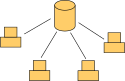
\includegraphics[width=0.7\textwidth]{01_centralized_vcs}
\end{figure}
\end{frame}

\begin{frame}{Centralized vs. Distributed VCS}{Centralized}
\begin{figure}
	\centering
	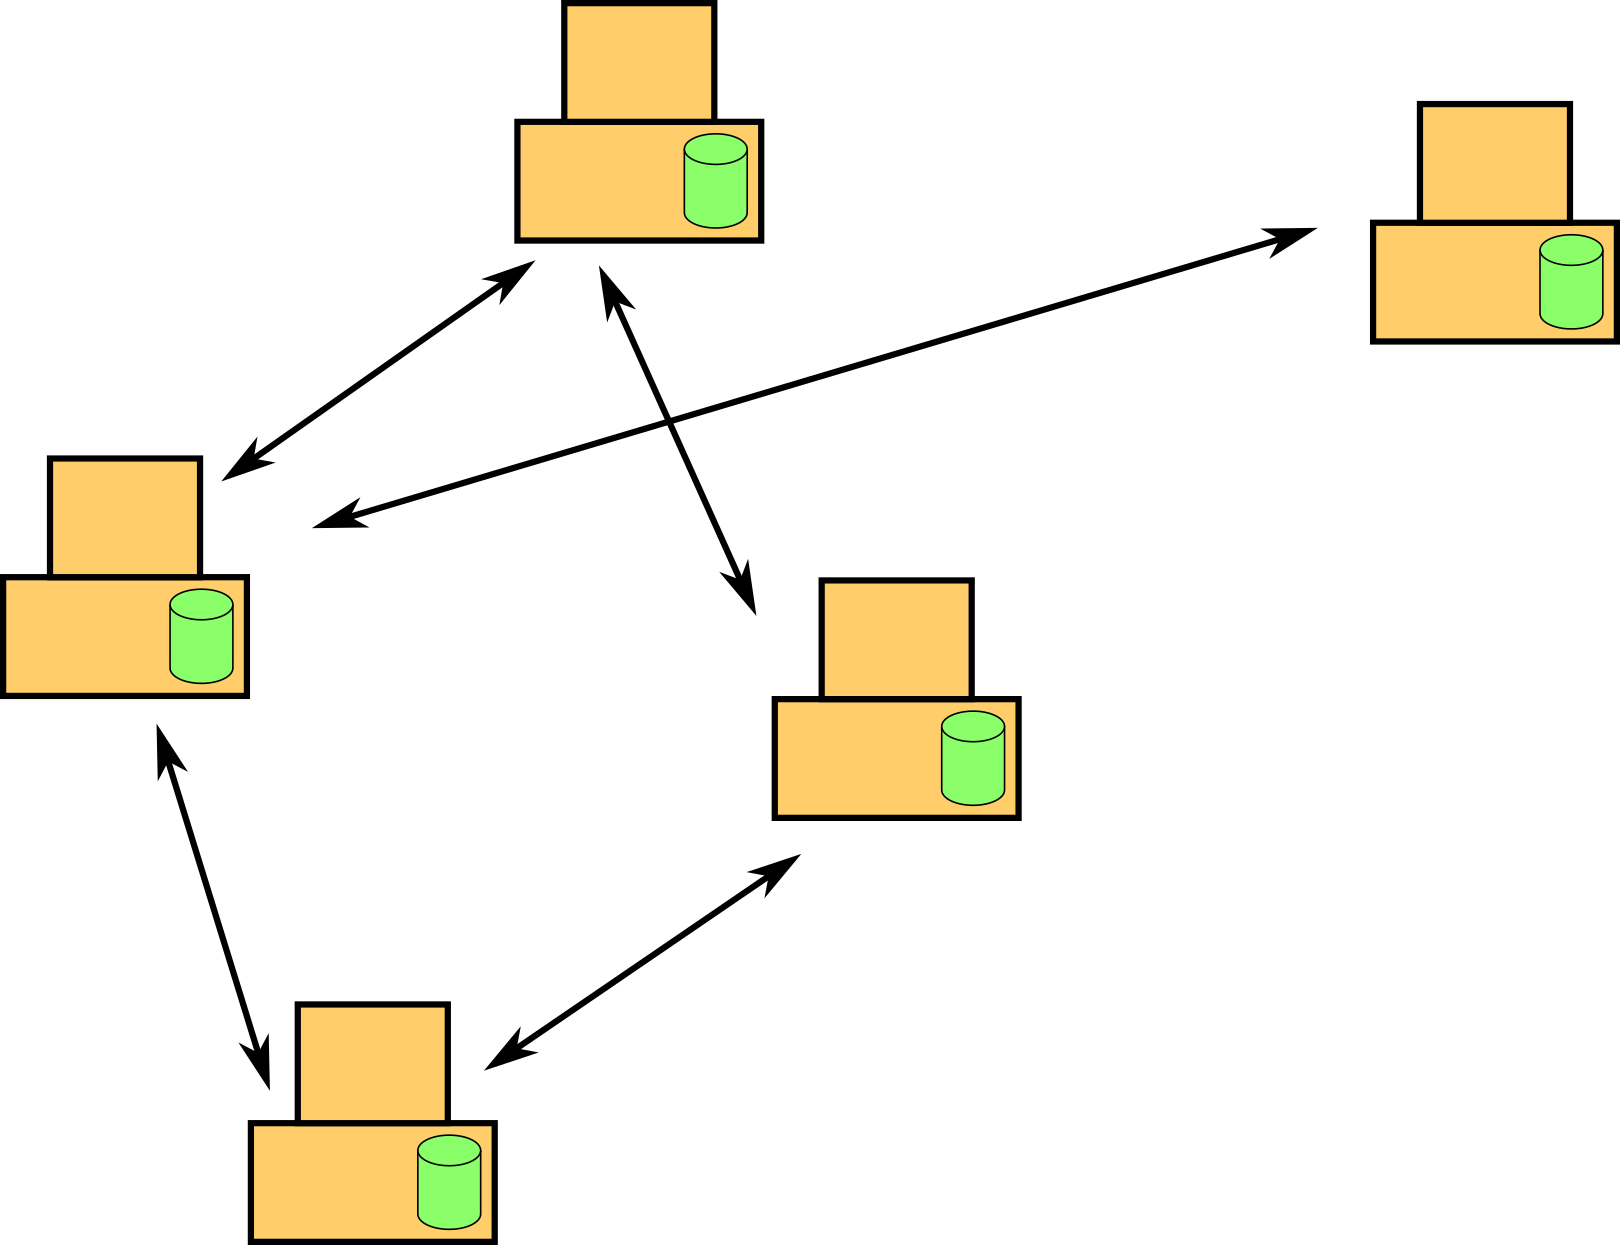
\includegraphics[width=0.6\textwidth]{02_distributed_vcs}
\end{figure}
\end{frame}

\begin{frame}{Deltas vs. Snapshots}{Deltas}
\begin{figure}
	\centering
	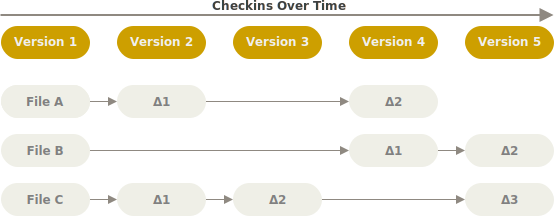
\includegraphics[width=1\textwidth]{deltas}
	\caption{
		Pro Git: 1.3 Getting Started - What is Git?\footnote{\url{https://git-scm.com/book/en/v2/Getting-Started-What-is-Git\%3F}}
	}
\end{figure}
\end{frame}

\begin{frame}{Deltas vs. Snapshots}{Snapshots}
\begin{figure}
	\centering
	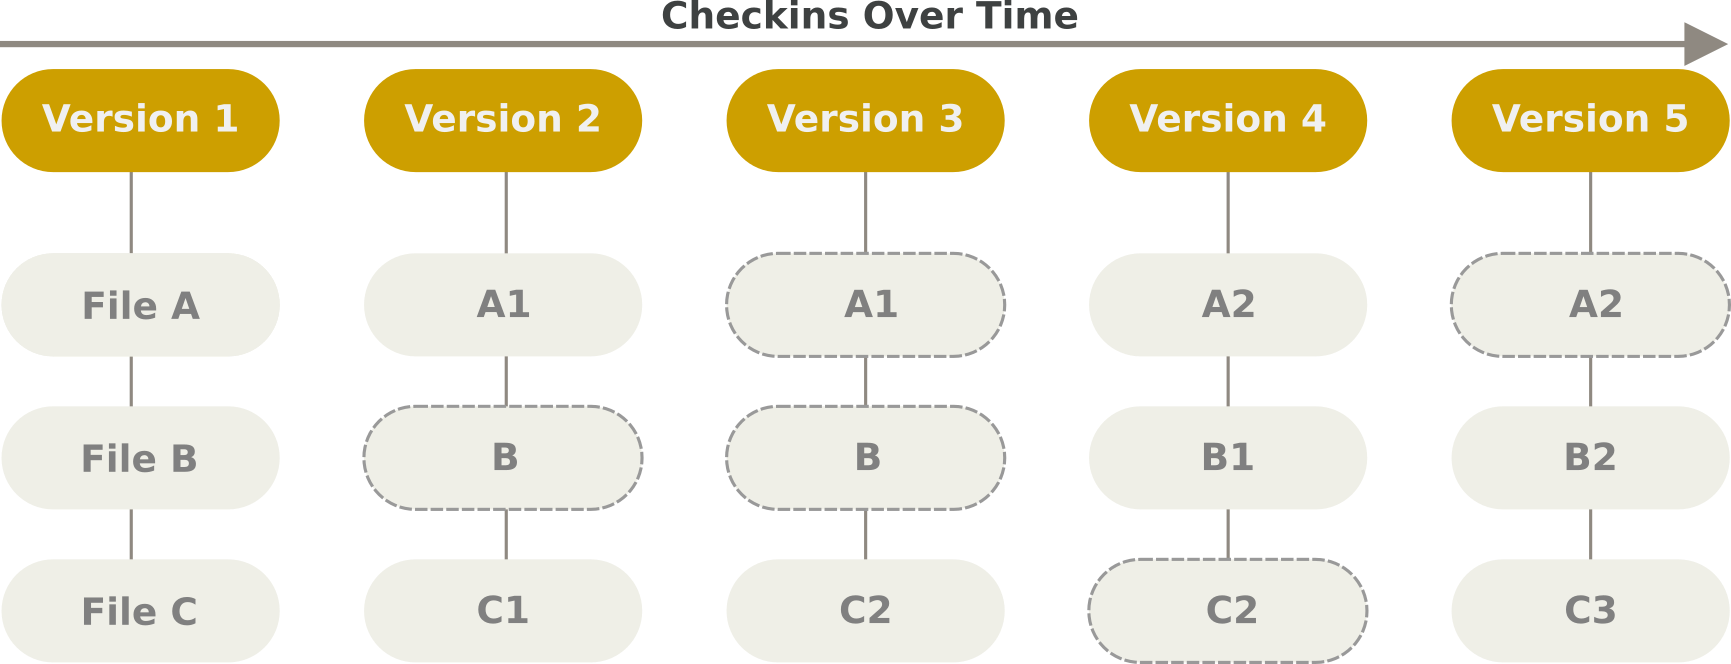
\includegraphics[width=1\textwidth]{snapshots}
	\caption{
		Pro Git: 1.3 Getting Started - What is Git?\footnote{\url{https://git-scm.com/book/en/v2/Getting-Started-What-is-Git\%3F}}
	}
\end{figure}
\end{frame}

\section{How does Git work?}
\begin{frame}[fragile]{How does Git Work?}{Every thing is a Hash}
\begin{minted}{bash}
$ sha1sum kunbus-logo.png 
c263869cf482a5d5d4262170ec242f8f13fc3def  kunbus-logo.png
$ ls -sh kunbus-logo.png 
352K kunbus-logo.png
\end{minted}
\begin{itemize}
	\item A file is an \emph{object} with a \emph{hash} and a \emph{size}
	\item Everything is identified by its hash, not only file objects
\end{itemize}
\end{frame}

\begin{frame}{How does Git Work?}{Git is a Tree of Hashes}
\begin{figure}
	\centering
	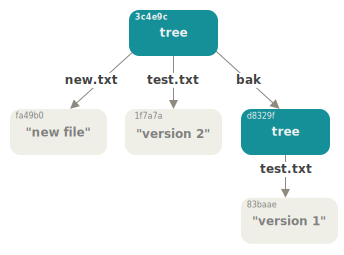
\includegraphics[width=0.5\textwidth]{data-model-2}
	\caption{
		Pro Git: 10.2 Git Internals - Git Objects\footnote{\url{https://git-scm.com/book/en/v2/Git-Internals-Git-Objects}}
	}
\end{figure}
\end{frame}

\begin{frame}{How does Git Work?}{Git is a Tree of Trees of Hashes}
\begin{figure}
	\centering
	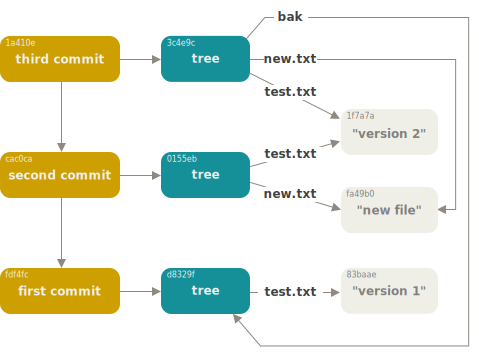
\includegraphics[width=0.5\textwidth]{data-model-3}
	\caption{
		Pro Git: 10.2 Git Internals - Git Objects\footnote{\url{https://git-scm.com/book/en/v2/Git-Internals-Git-Objects}}
	}
\end{figure}
\end{frame}

\section{The Basics}
\section{Not so Basic}
\section{Workflows}
\section{Github}

\end{document}
